PaxosKV's replicas need not share a datacenter. This chapter places
\texttt{kv0} and \texttt{kv1} in island \texttt{us} and \texttt{kv2} in island
\texttt{eu}, lets the replicas talk over UDP (as QUIC datagrams would), and asks
the LeanFM MCP server what that does to the protocol. Every verdict below is a
server answer kept in \texttt{reports/mcp/results.json}; the tables and
diagrams are typeset from that file by \texttt{scripts/mcp\_report.py}.

\section{The write as a session type}
\texttt{spec/Session.lean} states the write path with the
\texttt{LeanFM.Session} library. The leader \texttt{kv0} already holds a ballot
every replica has promised, so a write is phase~2 only: accept on two of three
replicas, durably, then answer. The leader's own acceptance is a local fsync, an
event at \texttt{kv0} alone.

% Generated by scripts/mcp_report.py from spec/Session.lean.
\begin{Verbatim}[fontsize=\small]
protocol QuorumWrite (Browser, Web, Kv0, Kv1, Kv2) {
  put:  PutRequest from Browser to Web;
  prop: Propose from Web to Kv0 cause put where prop.requestId = put.requestId;
  join 2 of {
    Fsync at Kv0;
  } and {
    a1: Accept from Kv0 to Kv1 cause prop;
        DurableAccepted from Kv1 to Kv0 cause a1;
  } and {
    a2: Accept from Kv0 to Kv2 cause prop;
        DurableAccepted from Kv2 to Kv0 cause a2;
  }
  res: PutResult from Kv0 to Web cause prop where res.requestId = prop.requestId;
       PutResponse from Web to Browser cause res;
}
\end{Verbatim}


The same file declares the physics and the deployment. Browser, web tier and
leader talk HTTP; replicas talk UDP to each other with capacity~8. The tree puts
the web tier and \texttt{kv0} on one machine in \texttt{us}, \texttt{kv1} on
another, and \texttt{kv2} alone in \texttt{eu}. Its \texttt{\#guard} lines are
checked whenever the file is elaborated:

\begin{itemize}\tightlist
\item the write and the takeover are well formed, and every role can tell which
  branch it is in;
\item every channel's conditions are handled by its protocol: UDP's loss,
  reordering and duplicates by ballots and retransmission, HTTP's timeouts and
  retried requests by \texttt{requestId};
\item the leader's internal API is open to the web tier and closed to the
  browser and to \texttt{kv2}; its peering port is open to \texttt{kv2};
\item a channel from \texttt{us} to \texttt{eu} surfaces \texttt{partition} as
  well, which the requirements do not yet mention.
\end{itemize}

The last point is the question for the server: what does a partition, or loss,
or reordering across the islands do to one Paxos slot?

\section{The model the server checks}
Most of PaxosKV needs no product at all. A role that forks one thread per
session, where each thread ingests only the messages its session expects and
sends only the ones it owes, can be checked one session at a time, and that is
exact rather than an approximation: no interleaving with another session can
change what one thread sees. Two browser writes are such sessions. The
leader's ballot and \texttt{kv2}'s takeover are not: they are different
sessions that meet in each acceptor's promised ballot and accepted value, state
that both read and write. That shared state is the only reason to build the
product, and it is all the product contains.

\texttt{spec/PaxosUdp.lean} builds the product of the three replicas and their
UDP channels for one slot. The leader \texttt{kv0} proposes \texttt{A} at
ballot~1. \texttt{kv2}, having lost touch with it, takes over with ballot~2:
phase~1, then the highest value its two promises report, or its own value
\texttt{B} if they report none. A sent message may reach each replica in any
order, late, or never; a learner reports \texttt{ChosenA} or \texttt{ChosenB}
when two replicas have accepted the same ballot and value. Four variants are
written as draft tasks for \texttt{check\_ctl}:

\begin{description}\tightlist
\item[\texttt{correct}] as above: 469 states, 1164 transitions.
\item[\texttt{broken}] \texttt{kv2} ignores what the promises report and
  proposes \texttt{B}: 547 states, 1309 transitions.
\item[\texttt{partitioned}] \texttt{correct}, with nothing crossing between
  \texttt{us} and \texttt{eu}.
\item[\texttt{lossy}] the leader alone, with every message free to be lost.
\end{description}

Loss needs care. Every prefix of a run that loses messages is also a prefix of
a run that only delays them, and the model delays any message arbitrarily, so
the safety verdicts hold for lossy UDP as they stand. Liveness does not
transfer: in the first three variants every message is eventually delivered,
which is the \texttt{fairDelivery} assumption written in the session spec. The
\texttt{lossy} variant drops that assumption on a slice small enough to carry
explicit \texttt{Lost} steps.

\section{What the server said}
Before checking, each formula was read back by \texttt{explain\_formula}. The
first draft of the agreement property used a plain implication; the server
warned that it would also hold if \texttt{ChosenA} never happened, so the
property uses \texttt{stronglyImplies}, as it suggested.

% Generated by scripts/mcp_report.py: explain_formula readings.
\begin{description}
\item[\texttt{agreement}] (ChosenA was just delivered can happen, and on every path, whenever ChosenA was just delivered then (on every path, always (it is not the case that ChosenB was just delivered))) and (ChosenB was just delivered can happen, and on every path, whenever ChosenB was just delivered then (on every path, always (it is not the case that ChosenA was just delivered))).
\item[\texttt{canDecide}] on every path, (it is possible that eventually (ChosenA was just delivered or ChosenB was just delivered)) holds unless (ChosenA was just delivered or ChosenB was just delivered) ((ChosenA was just delivered or ChosenB was just delivered) need not happen).
\item[\texttt{conflict}] it is possible that eventually (ChosenA was just delivered and (it is possible that eventually ChosenB was just delivered)).
\item[\texttt{mustDecide}] on every path, eventually (ChosenA was just delivered or ChosenB was just delivered).
\item[\texttt{possiblyA}] it is possible that eventually ChosenA was just delivered.
\item[\texttt{possiblyB}] it is possible that eventually ChosenB was just delivered.
\end{description}


% Generated by scripts/mcp_report.py from reports/mcp/results.json.
\begin{longtable}{@{}p{.13\textwidth}p{.27\textwidth}p{.11\textwidth}p{.43\textwidth}@{}}
\toprule
model & question & verdict & evidence \\
\midrule
\endhead
\texttt{broken} & no two different values are both chosen & \textbf{disproved} & counterexample: \texttt{Accept1A, Accepted1, ChosenA} \\
\texttt{broken} & A is chosen, and later B & \textbf{proved} & witness: \texttt{Accept1A, Accepted1, ChosenA, Prepare2, Promise0, Accept2B, Accepted0, ChosenB} \\
\texttt{correct} & no two different values are both chosen & \textbf{proved} & none, over all 1114 nodes \\
\texttt{correct} & until a value is chosen, one can still be chosen & \textbf{proved} & none, over all 1114 nodes \\
\texttt{correct} & A is chosen, and later B & \textbf{disproved} & none, over all 1114 nodes \\
\texttt{correct} & a value must be chosen & \textbf{proved} & none, over all 1114 nodes \\
\texttt{correct} & A can be chosen & \textbf{proved} & witness: \texttt{Accept1A, Accepted1, ChosenA} \\
\texttt{correct} & B can be chosen & \textbf{proved} & witness: \texttt{Prepare2, Promise0, Accept2B, Accepted0, ChosenB} \\
\texttt{lossy} & a value must be chosen & \textbf{disproved} & counterexample: \texttt{Accept1A, Lost, Lost, then nothing more} \\
\texttt{lossy} & A can be chosen & \textbf{proved} & witness: \texttt{Accept1A, Accepted1, ChosenA} \\
\texttt{partitioned} & until a value is chosen, one can still be chosen & \textbf{proved} & none, over all 11 nodes \\
\texttt{partitioned} & A can be chosen & \textbf{proved} & witness: \texttt{Accept1A, Accepted1, ChosenA} \\
\texttt{partitioned} & B can be chosen & \textbf{disproved} & none, over all 11 nodes \\
\bottomrule
\end{longtable}


\paragraph{Safety survives the islands.} With the correct takeover, no run
chooses two values, over all 1114 model nodes, whatever the order in which UDP
delivers the messages between \texttt{us} and \texttt{eu}. Both values are
possible on their own: \texttt{A} inside \texttt{us}, \texttt{B} when
\texttt{kv2} gets in first.

\paragraph{One line of the takeover is the whole difference.} With the broken
takeover the server returns a run that chooses both. It is short, and it crosses
the islands:

\begin{figure}[htbp]\centering
\ifdefined\darkmode
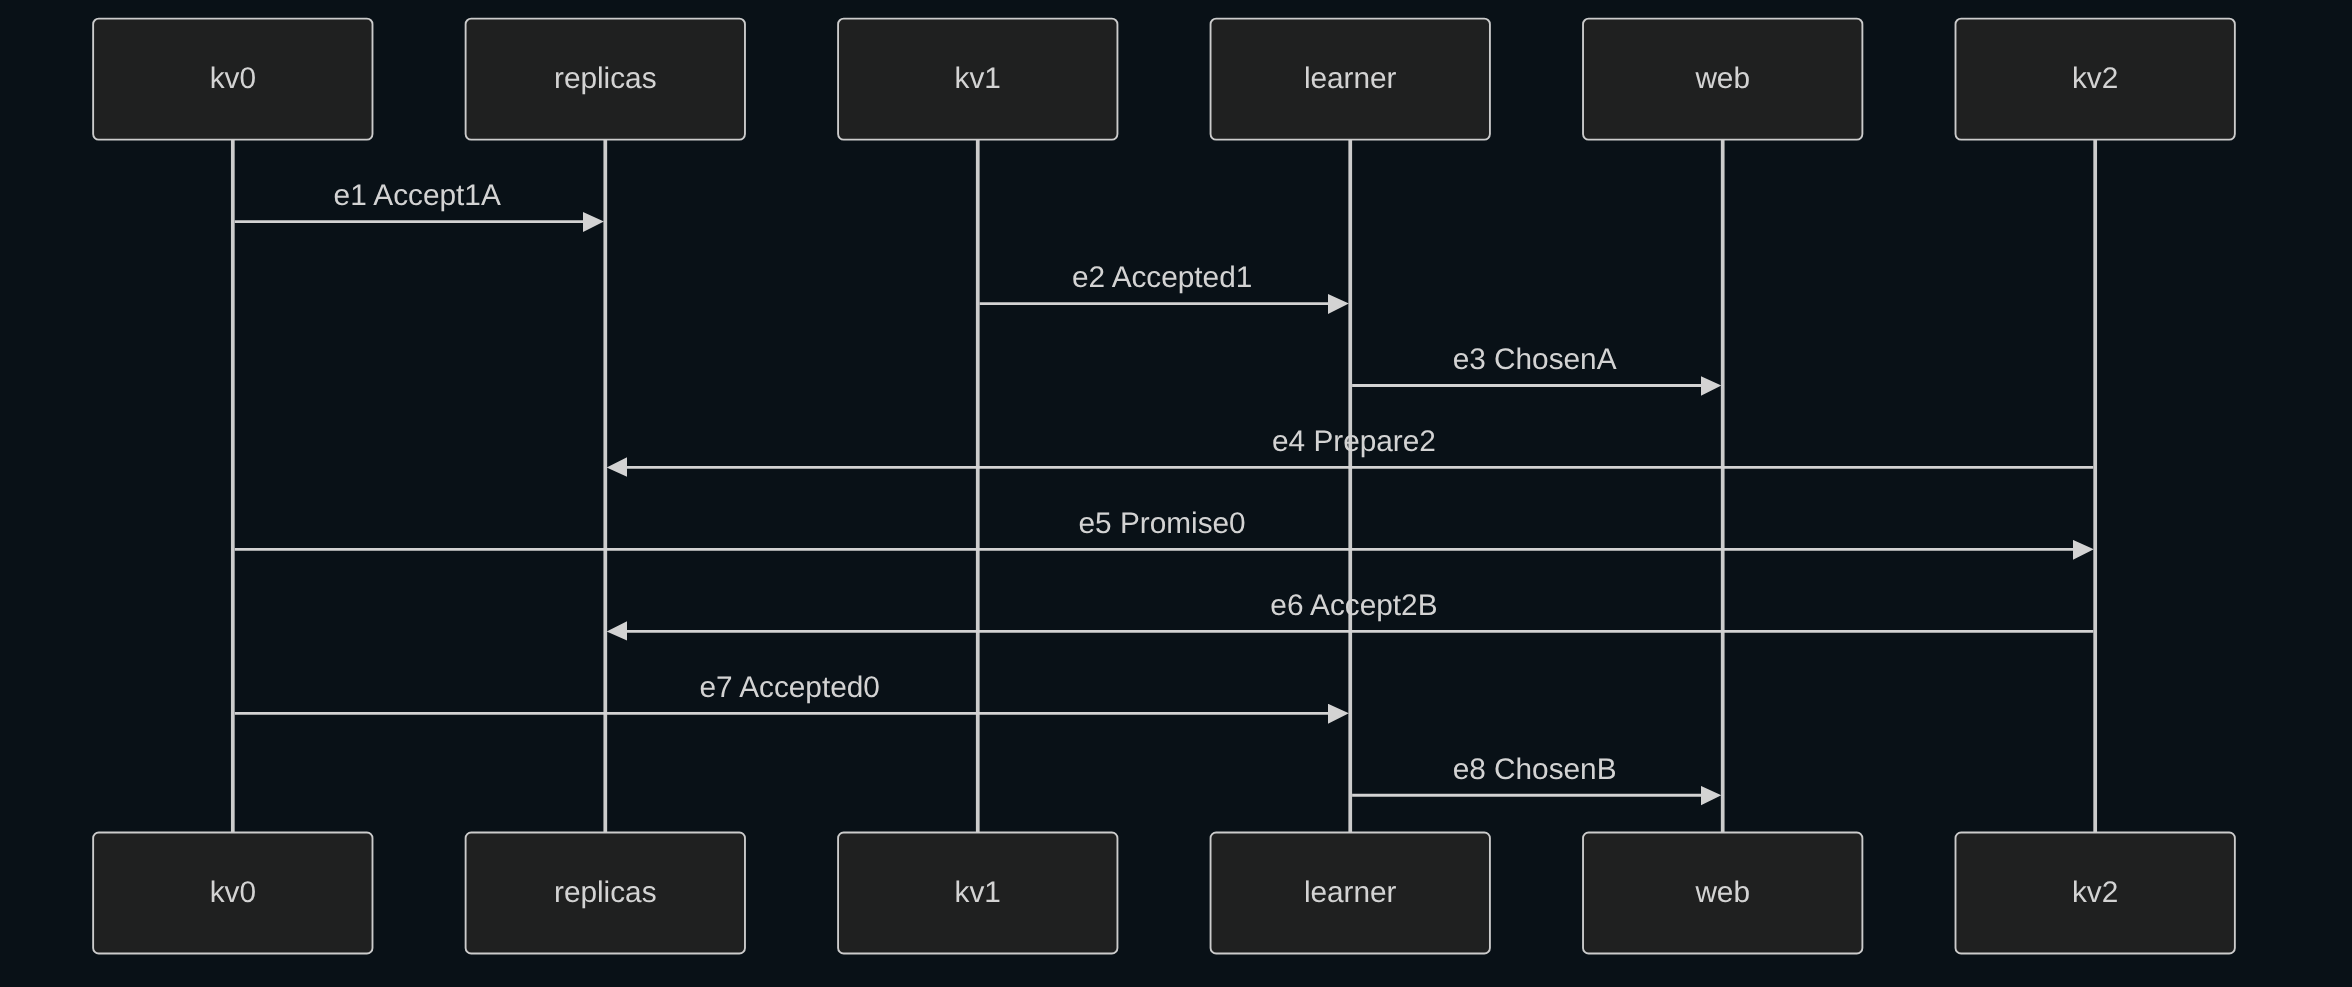
\includegraphics[width=\textwidth,height=0.42\textheight,keepaspectratio]{conflict-sequence-dark.png}
\else
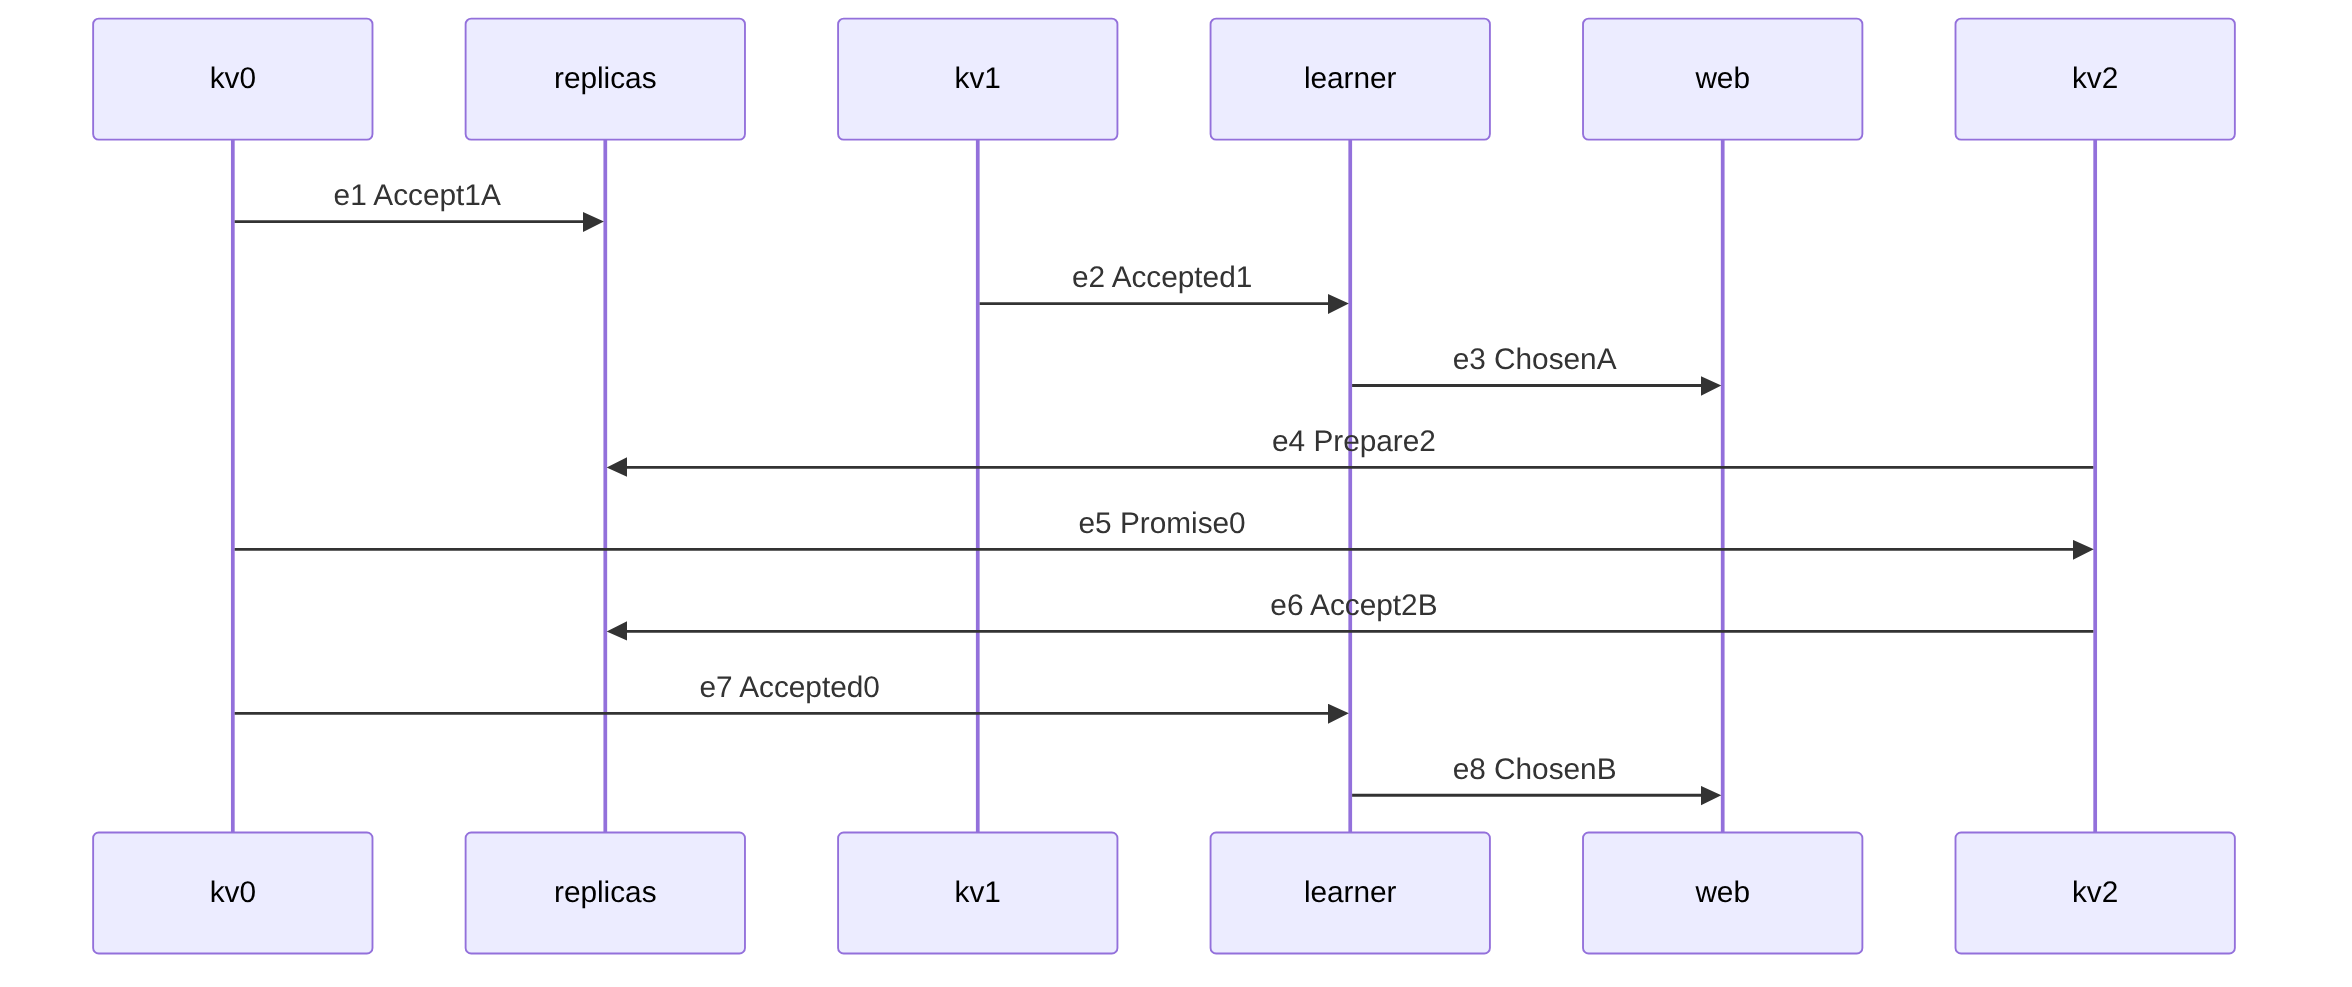
\includegraphics[width=\textwidth,height=0.42\textheight,keepaspectratio]{conflict-sequence.png}
\fi
\caption{The broken takeover, as \texttt{check\_trace} drew it from the
server's witness. \texttt{kv0} and \texttt{kv1} choose \texttt{A} inside
\texttt{us}. \texttt{kv2} then prepares ballot~2; \texttt{kv0}'s promise reports
that it accepted \texttt{A}, \texttt{kv2} ignores the report, and \texttt{kv0}
and \texttt{kv2} choose \texttt{B}.}
\end{figure}

The witness came in two questions. \texttt{check\_ctl} proves
$EF(\mathit{after}\ \mathit{ChosenA} \land EF\ \mathit{after}\ \mathit{ChosenB})$
with a path that stops where \texttt{ChosenA} holds; asking $EF\ \mathit{after}\
\mathit{ChosenB}$ again from that state gives the rest. \texttt{check\_trace}
then accepted the eight events, with their \texttt{prevIds} and
\texttt{causeIds}, and returned the sequence diagram above and the causal graph
below. It found nine concurrent pairs: the \texttt{us} decision and
\texttt{kv2}'s prepare are unordered, which is exactly why the takeover must
read the promises.

\begin{figure}[htbp]\centering
\ifdefined\darkmode
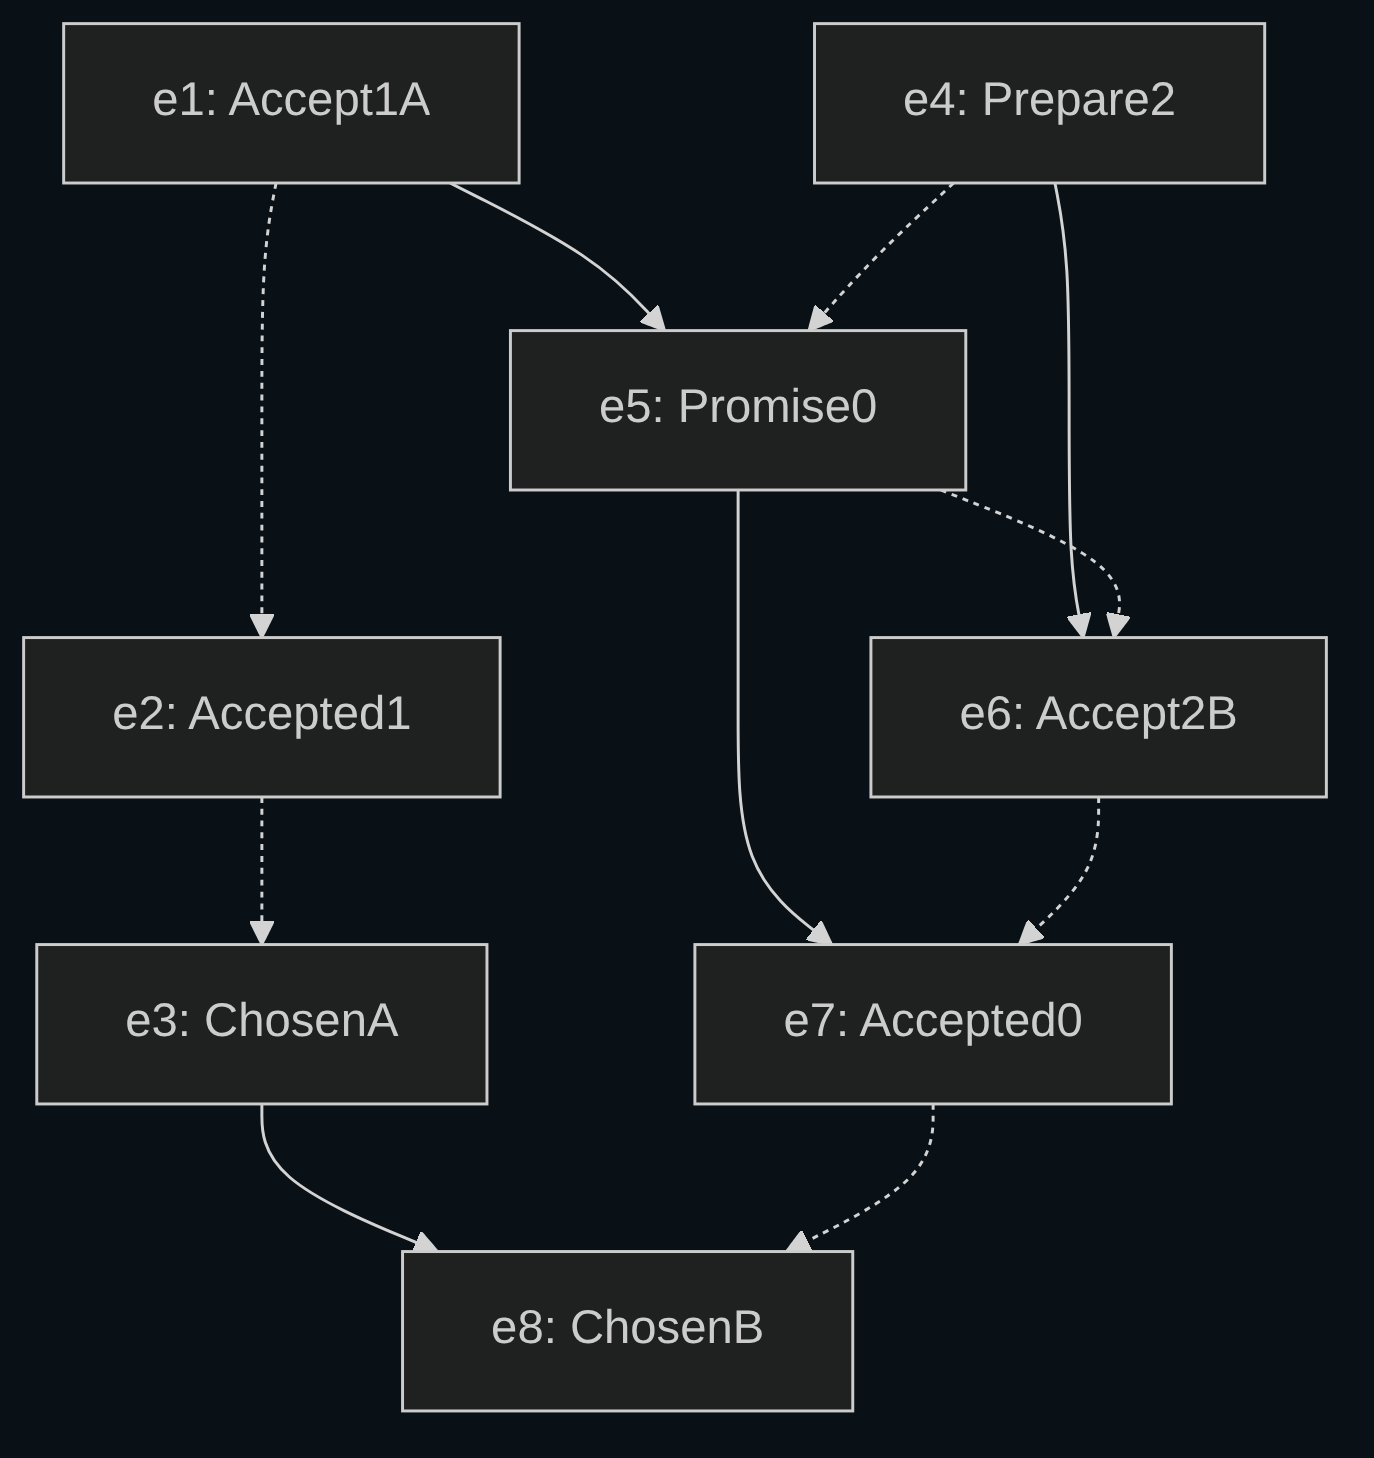
\includegraphics[width=0.55\textwidth,height=0.4\textheight,keepaspectratio]{conflict-causal-dark.png}
\else
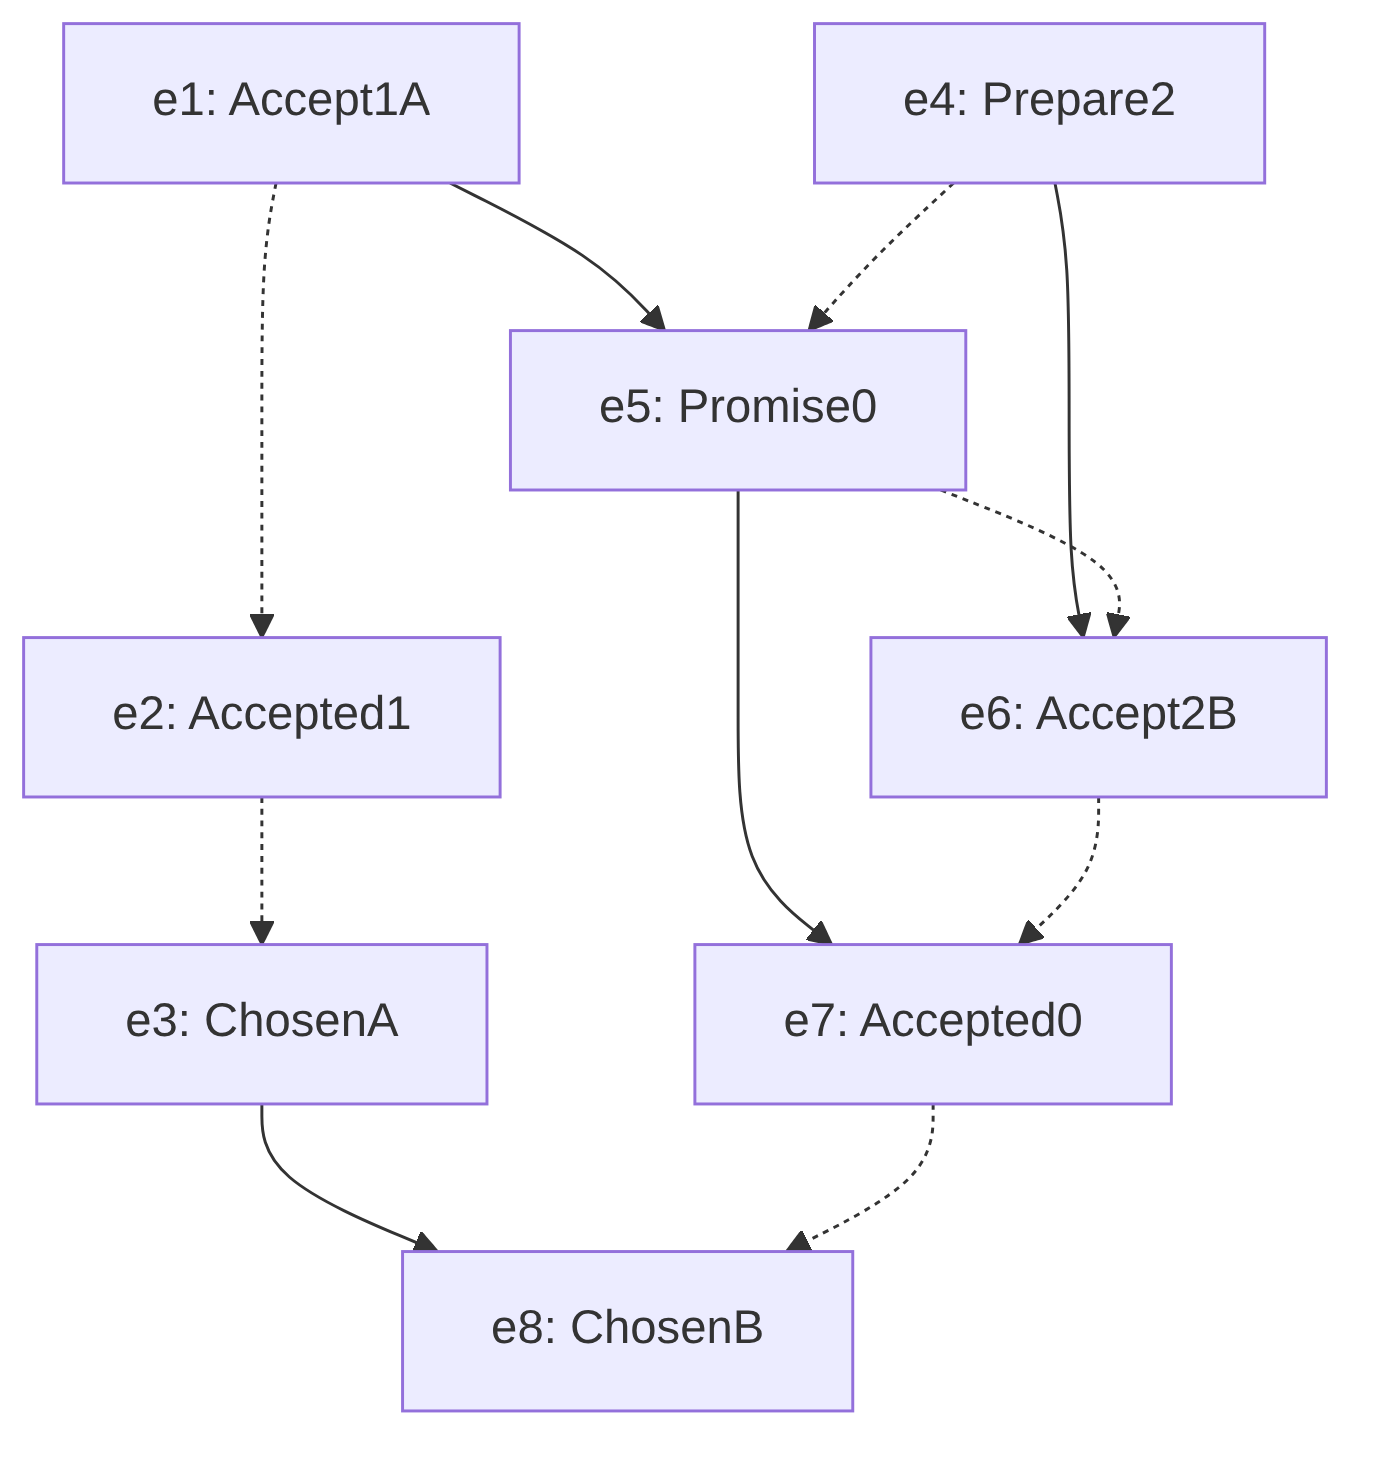
\includegraphics[width=0.55\textwidth,height=0.4\textheight,keepaspectratio]{conflict-causal.png}
\fi
\caption{Causal graph of the same run. Solid edges are \texttt{prevIds} (order
at one replica), dashed edges \texttt{causeIds}.}
\end{figure}

\paragraph{A partition leaves a quorum in \texttt{us}.} Cut \texttt{eu} off and
\texttt{A} can still be chosen; \texttt{B} cannot, over all 11 nodes. Until a
value is chosen one can always still be chosen, but only on the \texttt{us}
side: \texttt{kv2} alone is a minority.

\paragraph{Liveness needs fairness.} Under fair delivery a value must be chosen.
Drop fairness and the \texttt{lossy} slice returns the obvious lasso:
\texttt{Accept1A}, \texttt{Lost}, \texttt{Lost}, then nothing more. No protocol
can force UDP to deliver; the promise that a write completes rests on the
\texttt{fairDelivery} assumption, and on retransmission, which is a timer and
therefore physics.

\section{What cannot be observed}
\texttt{classify\_requirement} sorted three requirement sentences. The first is
how agreement is usually stated, and no event can test it; the server proposed
an event to expose it. The second restates it over the learner's events, which
makes it derived; the agreement formula above is that restatement, and every one
of its atoms is observable.

% Generated by scripts/mcp_report.py: classify_requirement answers.
\begin{description}
\item[implementation-only] the replicas in us and eu agree on the chosen value (proposes event \texttt{ReplicasUsEuObserved})
\item[derived] ChosenA and ChosenB are never both delivered
\item[implementation-only] kv2 has promised ballot 2 (proposes event \texttt{Kv2PromisedBallotObserved})
\item[observable] the agreement formula: every atom is observable; check\_ctl or check\_trace can decide it
\end{description}


\section{Reproducing this chapter}
With the LeanFM server running (\texttt{make serve} in the LeanFM root):
\begin{Verbatim}
cd ../..   # LeanFM root
lake build LeanFM.Session
lake env lean projects/PaxosKV/spec/Session.lean          # structural checks
lake env lean --run projects/PaxosKV/spec/PaxosUdp.lean   # draft tasks
cd projects/PaxosKV
python3 scripts/mcp_paxos_udp.py    # ask the server; reports/mcp/results.json
python3 scripts/mcp_report.py       # typeset tables and diagrams (mmdc)
make book
\end{Verbatim}
